\begin{frame}{Overview of electronic structure theory}
  \begin{itemize}
    \setlength\itemsep{0.1em}
    \item The goal of computational quantum chemistry is to find the solutions to the
          electronic time independent Schrodinger, which is an eigenvalue problem
          involving the {\color{red}electronic Hamiltonian}

          \begin{align*}
            & \hat{H}\Phi_{k} = (\hat{T}_{e}  + \hat{V}_{eN} + \hat{V}_{ee})\Phi_{k}  = E_{k}\Phi_{k}, \\
            & E_{0} < E_{1} < \ldots < E_{k} < \ldots
          \end{align*}

    \item Electronic wavefunction with lowest $E_{k}$ is called the
          {\color{red}ground} electronic state and the rest are referred to as
          {\color{red}excited} electronic states.

        \item Except for a few simple molecular systems like \ce{H} and \ce{H2^+},
          no analytical solutions exist. Hence, approximate methods
          based on the {\color{red}variational method}. (Szabo, 1982, p.31)
  \end{itemize}


  % where the eigenfunctions Φk({ri}; {RI }) correspond to electronic
  % wavefunctions and depend on the electron positions {ri} and parametrically
  % on the fixed nuclear positions {RI }.The indices k = 0, 1 . . . ∞ order the
  % eigenvalues Ek({RI })
  %
  % \begin{itemize}
  %   \setlength\itemsep{0.1em}
  %   \item A
  %   \item B
  % \end{itemize}

  % \annotate[yshift=3em]{above}{hbar}{$\hbar = \frac{h}{2\pi}$, reduced Planck constant}
  % \annotate[yshift=1em]{above}{Hhat}{Electronic Hamiltonian}
  % \annotate[yshift=1em]{above}{Tehat}{electron kinetic energy}
  % \annotate[yshift=1em]{below}{Venhat}{electron-nuclei Coulomb interaction}
  % \annotate[yshift=1em]{below}{Vehat}{electron-nuclei Coulomb interaction}
  % \annotatetwo[yshift=-1em]{below}{Psi2}{Psi3}{Wavefunction}

  % align involving the electronic Hamiltonian Hˆ Φk({ri}; {RI }) = Ek({RI})Φk({ri}; {RI }),
  % (2.2) where the eigenfunctions Φk({ri}; {RI }) correspond to electronic wavefunctions and
  % depend on the electron positions {ri} and parametrically on the fixed nuclear positions {RI }.
  % The indices k = 0, 1 . . . ∞ order the eigenvalues Ek({RI })

  % \renewcommand{\eqnhighlightheight}{\vphantom{\hat{H}}\mathstrut}
\end{frame}


\begin{frame}{Significance of ground state in quantum chemistry}
  \begin{itemize}
    \setlength\itemsep{0.1em}
    \item Ground state energy gives a grounding for excited state energies, as only energies differences (relative energies to the ground state) are measured experimentally.
    \item Energy differences between products and reactants determine thermodynamic stability.
    \item Binding energies are determined relative energies between a bound complex (typically ground state) and its separated form (excited state).
    \item A number of molecular properties (dipole moments, dipole polarizabilities, first hyperpolarizability, etc)
          can be determined as derivatives of the ground state energy.
    \item Minimizing the ground state energy with respect to geometry gives us a stable configuration of a molecule.
    % https://www2.chemistry.msu.edu/courses/cem888/harrison/topics_pdf/dipole_moment.pdf
    % https://chemistry.stackexchange.com/questions/152773/significance-of-the-ground-state-energy-in-quantum-chemistry
  \end{itemize}
\end{frame}

% \begin{frame}{Testing}
%   \begin{figure}
%     \centering
%     \begin{tikzpicture}[
%         box/.style={rectangle,draw,fill=gray!20,node distance=1cm,text width=15em,text centered,rounded corners,minimum height=0.1em,thick},
%         arrow/.style={draw,-latex',thick},
%         scale=0.25,
%       ]
%
%       \node [box] (potential) {$v_{\text{ext},s}(\vec r)=v_\text{H}(\vec r) + v_\text{xc}(\vec r) + v_\text{ext}(\vec r)$};
%       \node [box,below=0.5 of potential] (hamiltonian) {$\hat{H}_{KS}=-\frac{\hbar^2}{2m}\vec{\nabla}^2 + v_{\text{ext},s}(\vec r)$};
%       % \node [box,below=0.5 of hamiltonian] (se) {$\hat{H}_{KS} \phi_i(\vec r)= E_i \phi_i(\vec r)$};
%       % \node [box,below=0.5 of se] (density) {$\rho(\vec r)=\sum_{i=1}^n f_i\,|\phi_i(\vec r_i)|^2$};
%       \node [box,below=0.5 of density] (criterion) {Convergence criterion satisfied?};
%
%       \path
%       (potential.north west) ++(-1em,1em) coordinate (potential fit)
%       (criterion.south east) ++(1em,-1em) coordinate (criterion fit);
%
%       \node [box,above=1.5 of potential, fill=orange!30, text width=20em] (initial) {Supply initial density guess $\rho_\text{ini}(\vec r)$ to Kohn Sham equations};
%       \node [box,below=1.5 of criterion, fill=blue!30, text width=20em] (energy) {Use $\rho_\text{fin}(\vec r)$ to minimize total energy functional $E_{V_\text{ext}}[\rho]=T_{e,s}[\phi_i\{\rho\}] + V_{ee,H}[\rho] + E_{xc}[\rho] + V_{eI}[\rho]$};
%
%       % \path [arrow] (initial) -- (potential);
%       % \path [arrow] (potential) -- (hamiltonian);
%       % \path [arrow] (hamiltonian) -- (se);
%       % \path [arrow] (se) -- (density);
%       % \path [arrow] (density) -- (criterion);
%
%       \node [rectangle,draw,dashed,inner sep=1em,fit=(potential fit) (criterion fit)] (enclosure) {};
%       \node [above=-0.8em of enclosure,anchor=south,draw,outer sep=0pt,fill=white] (enclosure label) {\Large\textbf{Kohn-Sham method}};
%
%       \path [arrow] (criterion) -- (energy) node [midway,left=0.1,draw,outer sep=0pt,fill=white] (TextNode) {Yes};
%       \path [draw,thick] (criterion.south) ++(0em,-1em) -- (criterion fit) node [midway,below=0.1,sloped,draw,outer sep=0pt,fill=white] (TextNode) {No};
%       \draw [arrow] (criterion fit) |- (potential.east);
%     \end{tikzpicture}
%   \end{figure}
% \end{frame}

\begin{frame}{Overview of variational method}
  For any valid and normalized approximate wavefunction $\tilde{\Phi}$, it holds that {\color{red} $C[\tilde{\Phi}] =  {\ev*{\hat{H}}{\tilde{\Phi}}} \geq E_{0}$}
  i.e. the energy of an approximate wavefunction will be above the true ground state energy. This gives a powerful procedure for finding
  estimating the true ground state energy:

  \begin{itemize}
    \setlength\itemsep{0.1em}
    \item Pick an {\color{red}ansatz} for the trial wave function $\ket{\tilde{\Phi}(\boldsymbol{\theta})}$.
    \item Systematically vary the parameters $\boldsymbol{\theta}$ and compute $E = \ev*{\hat{H}}{\tilde{\Phi}(\boldsymbol{\theta})}$.
    \item Repeat above step until $\tilde{E} = \ev*{\hat{H}}{\tilde{\Phi}(\boldsymbol{\theta})}$ settles on a minimum.
          This minimum will be our estimate of the true ground state energy.
  \end{itemize}
\end{frame}

% \begin{frame}{Preliminaries}
%     \begin{figure}
%       \centering
%       \includegraphics[width=1\linewidth]{h2o_symmetric_pes.pdf}
%       \caption{
%         Potential energy surface (PES) of water molecule along the reaction coordinate R,
%         which parameterizes the radial interatomic distance between the two hydrogen
%         atoms and the oxygen atom.
%       }
%     \end{figure}
% \end{frame}

\begin{frame}{Overview of electronic structure classical methods}
  \def\range{8}
  \def\xyRatio{2/3}
  \def\circSize{1mm}

  \begin{figure}
    \centering
    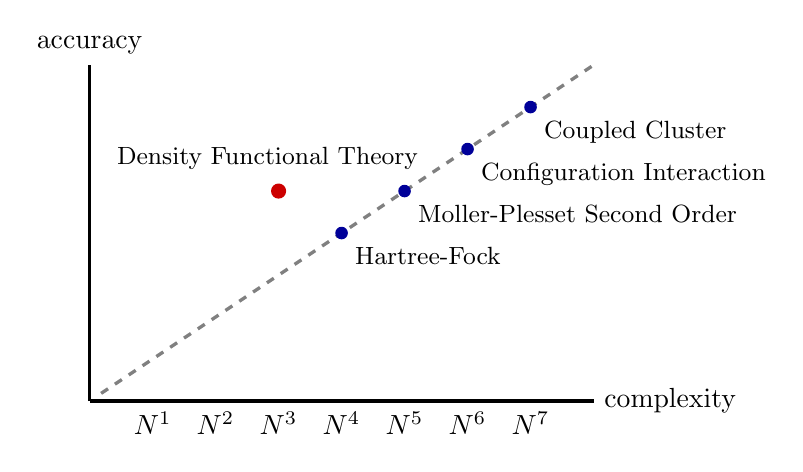
\begin{tikzpicture}[-, very thick, align=center, scale=0.8]
      \draw (0,0) -- (0,\range*\xyRatio) node[above] {accuracy};
      \draw (0,0) -- (\range,0) node[right] {complexity};
      \foreach \n in {1,...,7}
      \node[below] at (\n,0) {$N^\n$};

      \draw[dashed, gray, shorten <=5] (0,0) -- (\range,\range*\xyRatio);

      \foreach \n/\name/\abbr in {4/Hartree-Fock/HF, 5/Moller-Plesset Second Order/MP2, 6/Configuration Interaction/CISD, 7/Coupled Cluster/CCSD(T)}
      \fill[blue!60!black] (\n,\xyRatio*\n) circle (\circSize)
      node[align=left, below right=1pt, black] (\abbr) {\small\name};

      % \draw[red, thick] (HF) -- (SE);

      \fill[red!80!black] (3,5*\xyRatio) circle (1.2*\circSize) node[above=4pt, xshift=-4pt, black] (DFT) {\small Density Functional Theory};
      % \fill[blue!60!black] (4.5,6.5*\xyRatio) circle (\circSize) node[left=1ex, black] {Deep QMC};
    \end{tikzpicture}
    \caption{
      Cost vs accuracy trade-off for different quantum mechanics approximations. $N$ denotes the number of electrons.
      Adapted from \href{https://tikz.janosh.dev/qm-cost-vs-acc}{here}.
    }
  \end{figure}
\end{frame}

\begin{frame}{Overview of variational quantum eigensolver}
    \begin{figure}
      \centering
      \includegraphics[height=0.65\textwidth]{vqe_flowchart.pdf}
      \caption{Schematic for VQE pipeline.}
    \end{figure}
\end{frame}
